\documentclass{article}
\usepackage{tikz}
\usepackage{amsmath}
\usepackage{amssymb} % for logic symbols

\begin{document}

% ---------------- Conjunction ----------------
\begin{center}
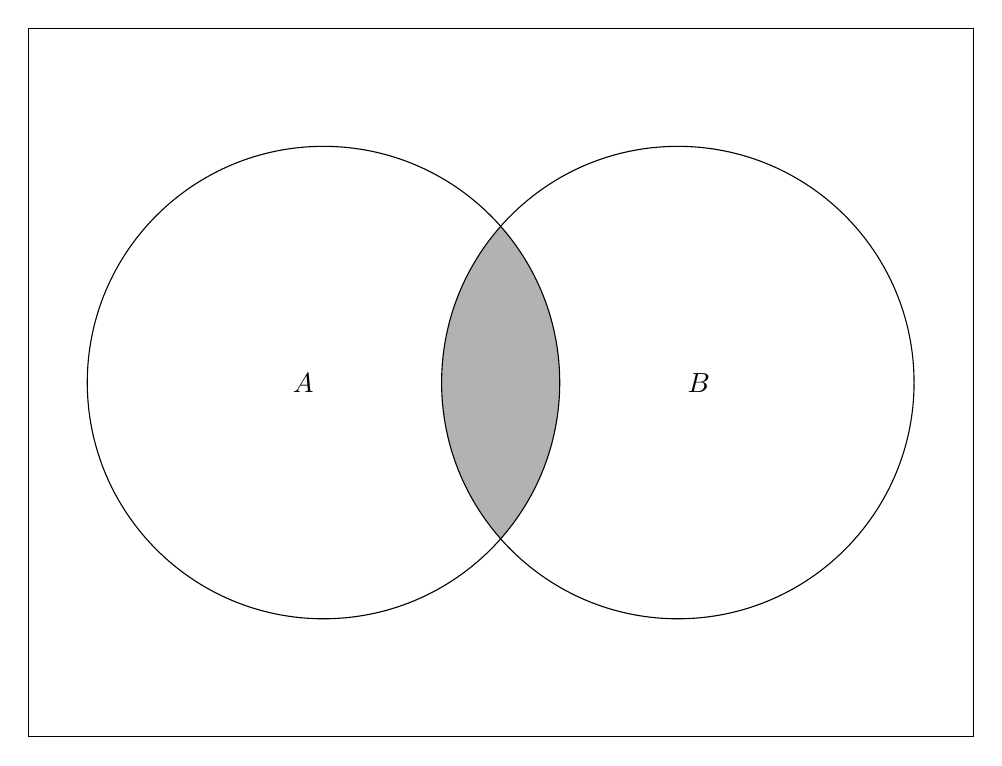
\begin{tikzpicture}[scale=3]
  % Shading first
  \begin{scope}
    \clip (-0.75,0) circle (1cm);
    \fill[gray!60] (0.75,0) circle (1cm);
  \end{scope}
  % Box and circles
  \draw (-2,-1.5) rectangle (2,1.5);
  \draw (-0.75,0) circle (1cm) node[left] {$A$};
  \draw (0.75,0) circle (1cm) node[right] {$B$};
\end{tikzpicture}

\[
A \wedge B
\]
\end{center}
\vspace{2cm}

% ---------------- Disjunction ----------------
\begin{center}
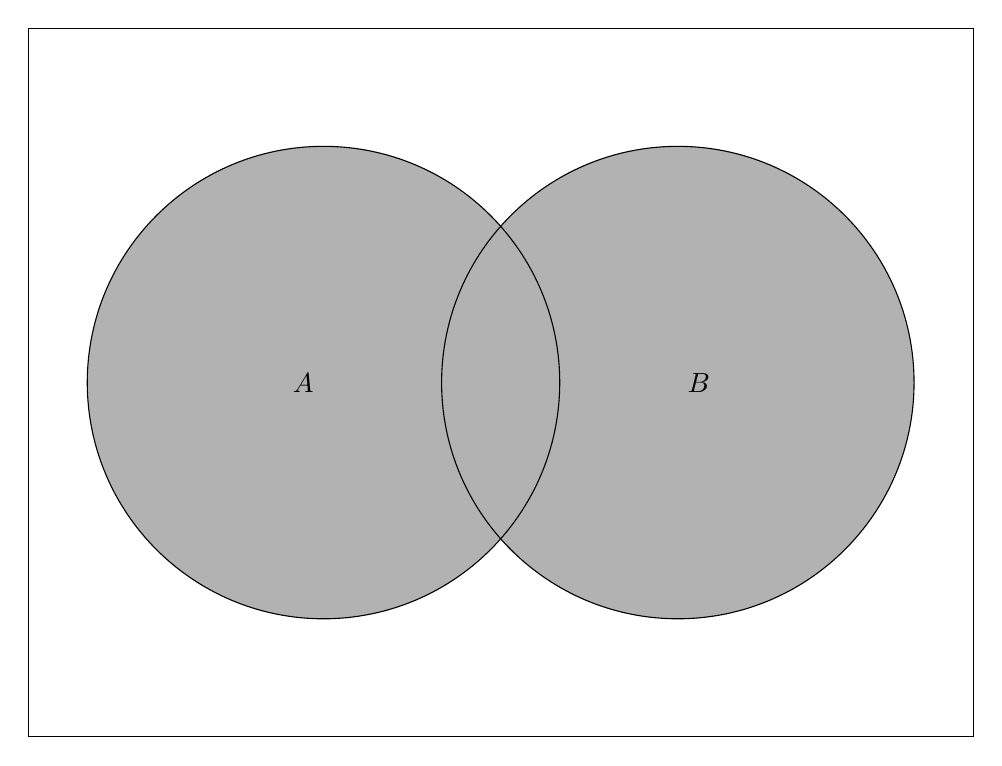
\begin{tikzpicture}[scale=3]
  % Shading
  \fill[gray!60] (-0.75,0) circle (1cm);
  \fill[gray!60] (0.75,0) circle (1cm);
  % Box and circles
  \draw (-2,-1.5) rectangle (2,1.5);
  \draw (-0.75,0) circle (1cm) node[left] {$A$};
  \draw (0.75,0) circle (1cm) node[right] {$B$};
\end{tikzpicture}

\[A \vee B\]

\end{center}
\vspace{2cm}

% ---------------- Negation ----------------
\begin{center}
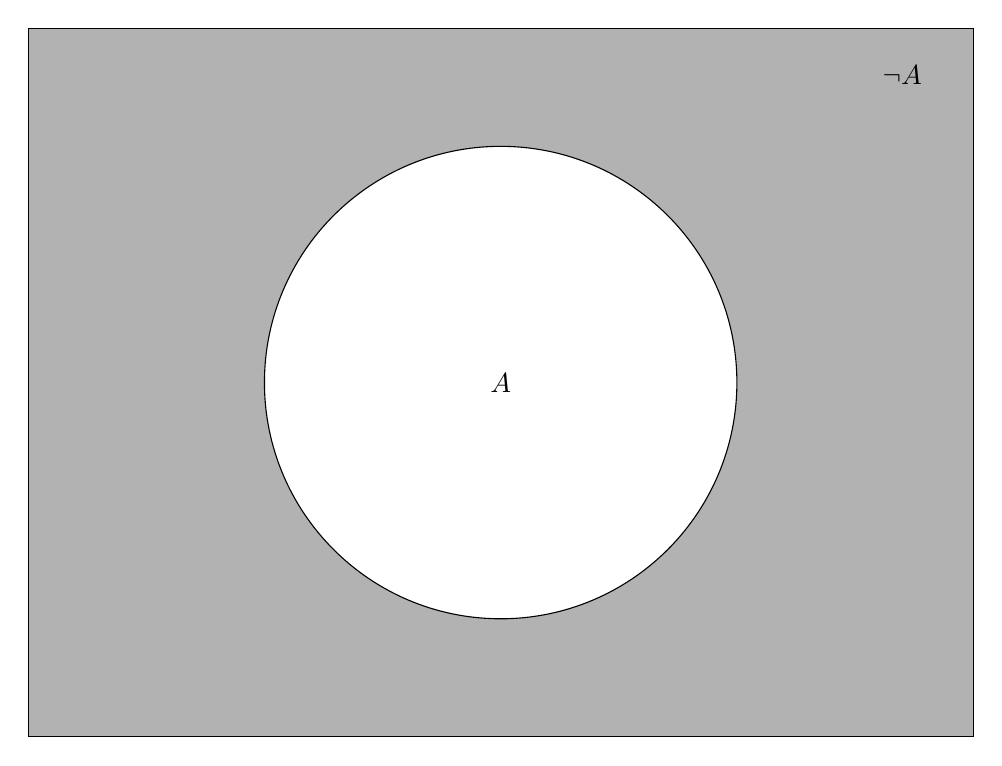
\begin{tikzpicture}[scale=3]
  % Shade everything
  \fill[gray!60] (-2,-1.5) rectangle (2,1.5);
  % Remove A
  \fill[white] (0,0) circle (1cm);
  % Draw box + circle
  \draw (-2,-1.5) rectangle (2,1.5);
  \draw (0,0) circle (1cm) node {$A$};
  \node at (1.7,1.3) {$\neg A$};
\end{tikzpicture}

\[
\neg A
\]
\end{center}
\vspace{2cm}

% ---------------- Implication ----------------
\begin{center}
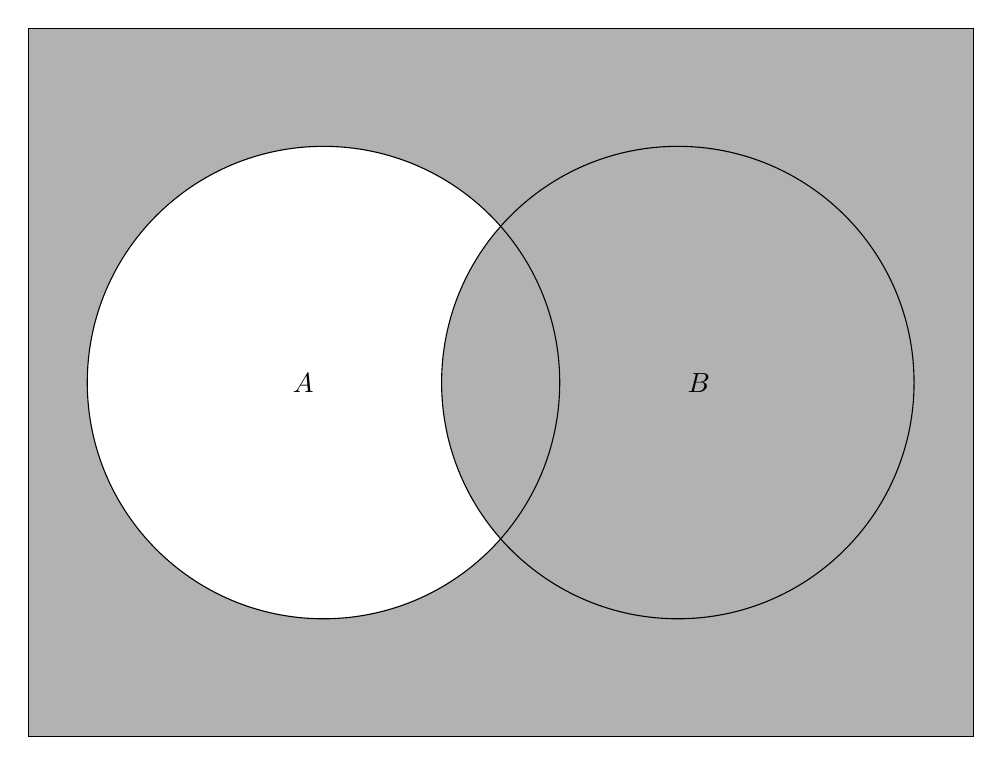
\begin{tikzpicture}[scale=3]
  % Shade full universe
  \fill[gray!60] (-2,-1.5) rectangle (2,1.5);
  % Remove A
  \fill[white] (-0.75,0) circle (1cm);
  % Add back A ∧ B
  \begin{scope}
    \clip (-0.75,0) circle (1cm);
    \fill[gray!60] (0.75,0) circle (1cm);
  \end{scope}
  % Box and circles
  \draw (-2,-1.5) rectangle (2,1.5);
  \draw (-0.75,0) circle (1cm) node[left] {$A$};
  \draw (0.75,0) circle (1cm) node[right] {$B$};
\end{tikzpicture}

\[
A \to B
\]
\end{center}
\vspace{2cm}

% ---------------- Negation of Conjunction ----------------
\begin{center}
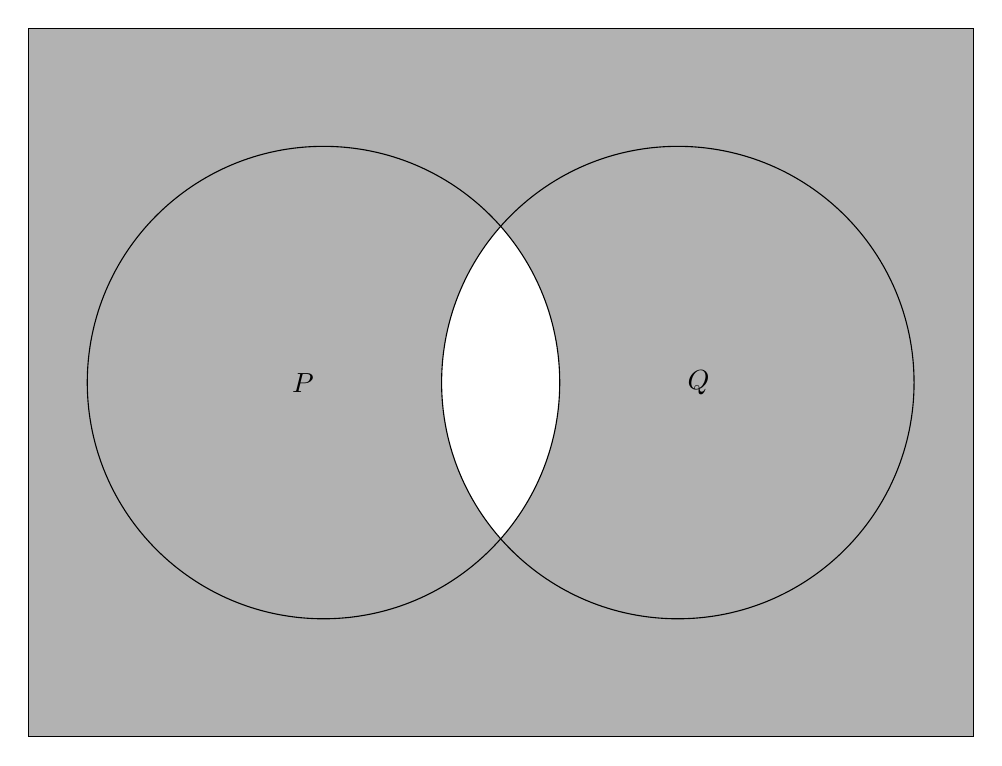
\begin{tikzpicture}[scale=3]
  % Shade everything
  \fill[gray!60] (-2,-1.5) rectangle (2,1.5);
  % Remove ONLY intersection
  \begin{scope}
    \clip (-0.75,0) circle (1cm);
    \fill[white] (0.75,0) circle (1cm);
  \end{scope}
  % Box and circles
  \draw (-2,-1.5) rectangle (2,1.5);
  \draw (-0.75,0) circle (1cm) node[left] {$P$};
  \draw (0.75,0) circle (1cm) node[right] {$Q$};
\end{tikzpicture}

\[
\neg (P \wedge Q) \;\equiv\; (\neg P) \vee (\neg Q)
\]
\end{center}
\vspace{2cm}

% ---------------- (~P) ∧ Q ----------------
\begin{center}
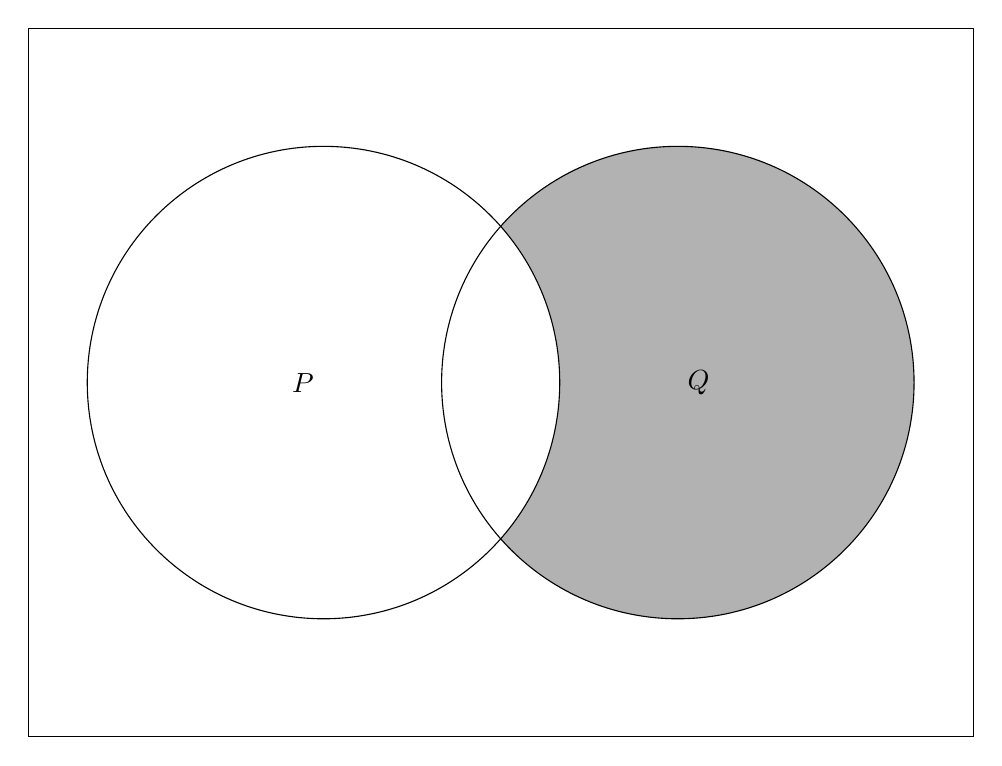
\begin{tikzpicture}[scale=3]
  % Shade Q first
  \fill[gray!60] (0.75,0) circle (1cm);
  % Remove intersection with P
  \begin{scope}
    \clip (-0.75,0) circle (1cm);
    \fill[white] (0.75,0) circle (1cm);
  \end{scope}
  % Box and circles
  \draw (-2,-1.5) rectangle (2,1.5);
  \draw (-0.75,0) circle (1cm) node[left] {$P$};
  \draw (0.75,0) circle (1cm) node[right] {$Q$};
\end{tikzpicture}

\[
(\neg P) \wedge Q
\]
\end{center}
\vspace{2cm}

% ---------------- Three propositions: Conjunction ----------------
\begin{center}
\textbf{Conjunction of Three Propositions:} Shade only the area where all three overlap.
\begin{tikzpicture}[scale=2.5]
  % Shade intersection A ∧ B ∧ C
  \begin{scope}
    \clip (-1,0) circle (1cm);   % A
    \clip (1,0) circle (1cm);    % B
    \clip (0,-0.7) circle (1cm); % C
    \fill[gray!60] (-1,0) circle (1cm);
  \end{scope}

  % Draw box and circles
  \draw (-3,-2) rectangle (3,2);
  \draw (-1,0) circle (1cm) node[left] {$A$};
  \draw (1,0) circle (1cm) node[right] {$B$};
  \draw (0,-0.7) circle (1cm) node[below] {$C$};
\end{tikzpicture}

\[
A \wedge B \wedge C
\]
\end{center}
\vspace{2cm}

% ---------------- Three propositions: Disjunction ----------------
\begin{center}
\textbf{Disjunction of Three Propositions:} Shade all areas inside any circle.
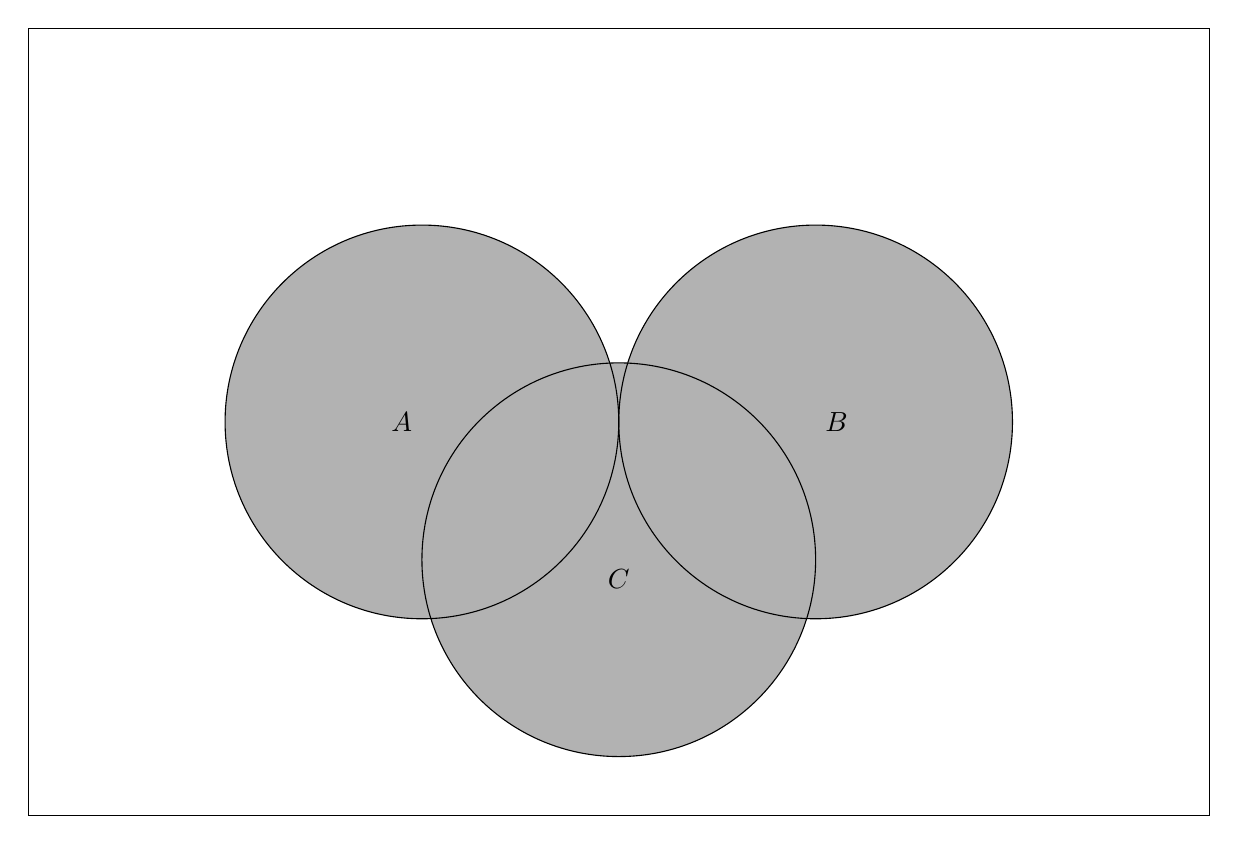
\begin{tikzpicture}[scale=2.5]
  % Shade A ∨ B ∨ C
  \fill[gray!60] (-1,0) circle (1cm);
  \fill[gray!60] (1,0) circle (1cm);
  \fill[gray!60] (0,-0.7) circle (1cm);

  % Draw box and circles
  \draw (-3,-2) rectangle (3,2);
  \draw (-1,0) circle (1cm) node[left] {$A$};
  \draw (1,0) circle (1cm) node[right] {$B$};
  \draw (0,-0.7) circle (1cm) node[below] {$C$};
\end{tikzpicture}

\[
A \vee B \vee C
\]
\end{center}
\vspace{2cm}

% ---------------- Three propositions: Negation of Conjunction ----------------
\begin{center}
\textbf{Negation of Conjunction:} Shade everything except the triple intersection.
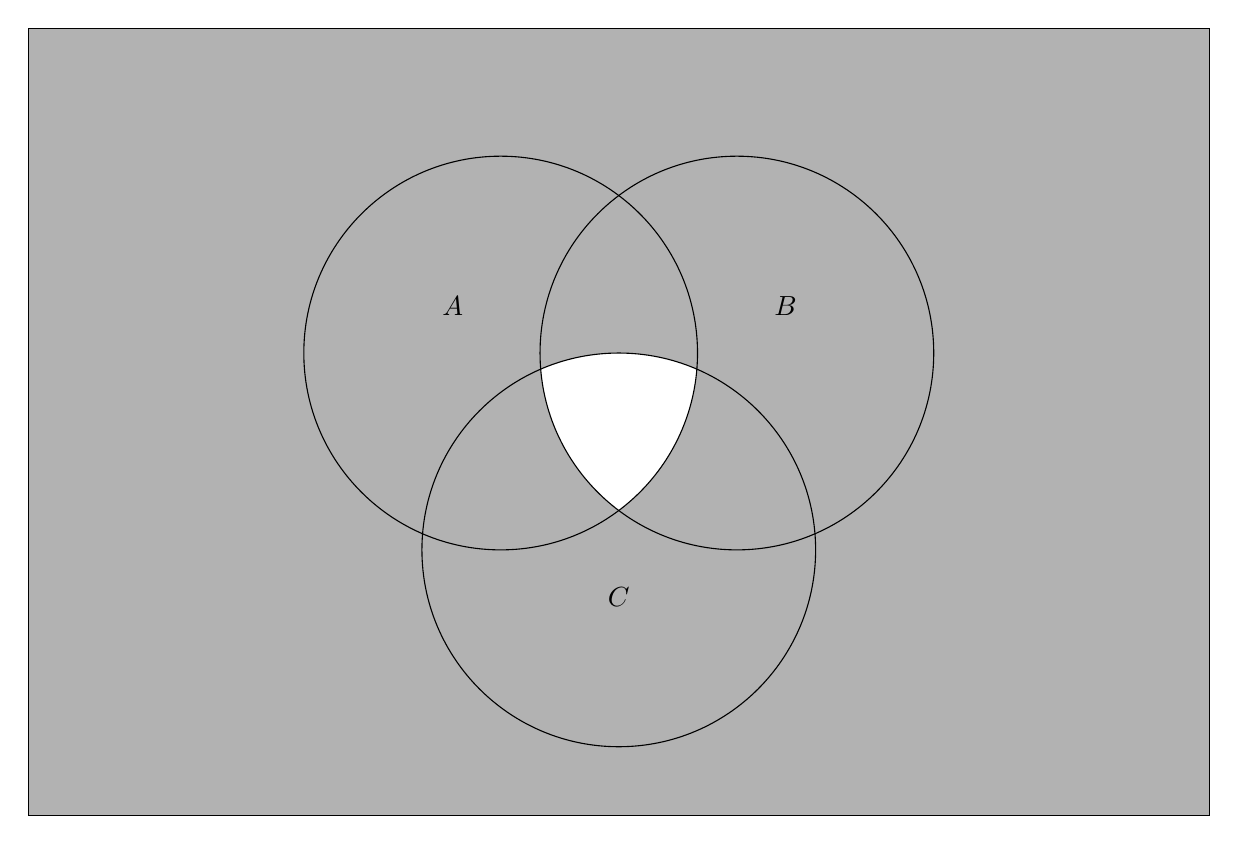
\begin{tikzpicture}[scale=2.5]
  % Shade entire universe
  \fill[gray!60] (-3,-2) rectangle (3,2);

  % Remove intersection A ∧ B ∧ C
  \begin{scope}
    \clip (-0.6,0.35) circle (1cm);
    \clip (0.6,0.35) circle (1cm);
    \clip (0,-0.65) circle (1cm);
    \fill[white] (-3,-2) rectangle (3,2); % shade triple overlap with white
  \end{scope}

  % Draw box
  \draw (-3,-2) rectangle (3,2);

  % Draw three circles centered symmetrically
% Draw three circles with custom label positions
\draw (-0.6,0.35) circle (1cm) node[above left, xshift=-10pt, yshift=10pt] {$A$};
\draw (0.6,0.35) circle (1cm) node[above right, xshift=10pt, yshift=10pt] {$B$};
\draw (0,-0.65) circle (1cm) node[below, yshift=-10pt] {$C$};


\end{tikzpicture}

\[
\neg(A \wedge B \wedge C) \;\equiv\; (\neg A) \vee (\neg B) \vee (\neg C)
\]

\end{center}
\vspace{2cm}


\end{document}
